\documentclass{article}

\usepackage[margin=1.0in]{geometry}
\usepackage{graphicx}
\usepackage{amsmath}
\usepackage{float}
\usepackage{enumitem}
\usepackage{gensymb}

\title{CSC 577 HW2}
\date{1/23/2019}
\author{Simon Swenson}

\begin{document}

\pagenumbering{gobble}
\maketitle
\pagenumbering{arabic}

\section{Introduction}

The main goal of this assignment was to get more familiar with spectral samples, 
sensors, the resultant RGB values, and the interplay between those three 
variables. The main activity was exploring methods of solving 
linear equations with multiple solutions and applying those methods to solve for 
hidden sensor sensitivities. I found sifting through the large amount of plots and
error values  for the undergraduate section tedious, but the concepts introduced in the graduate section 
were really cool. All problems were completed.

\section{(\#1) The Setup and Visualization}

\begin{figure}[!ht]
	\centering
	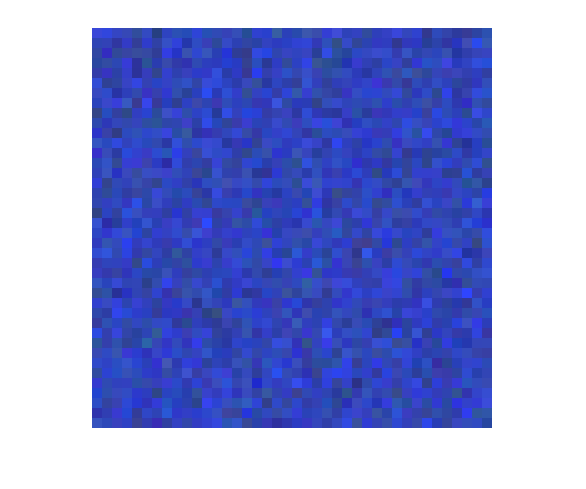
\includegraphics[width=120mm]{figs/image.png}
	\caption{Sensor responses (RGB values) for a randomly generated set of 1600 spectra, laid out in a 40 x 40 grid.}
\end{figure}

This portion of the assignment really just involved reading in the data, performing the 
standard spectra times sensor operation, and visualizing the resultant RGB values. 
The assignment mentioned that the sensors were biased toward blue, but I did not 
expect such a large bias! There are very few hues in here that one could consider 
\textit{not} blue. I see a few desaturated blue grays and aquas, though.

\section{(\#2) Predicting Sensors from Perfect Output Data}

Now that we have the data, we can start exploring different ways to manipulate it. 
First, we pretend that we do not have the original sensor sensitivity data, and 
we try to recover it from the sensor responses (RGB values). Recall that, with 
no error, we could solve the linear system of equations by simply multiplying 
the RGB on the left by the inverse of the spectra matrix. The pseudoinverse 
method is instead used, since we have more spectral samples than spectral 
wavelength buckets. This has the handy side-effect that the output is also the 
solution with the lowest mean squared error.

In the case of perfect output (no noise or clipping), we'll find that the error 
is extremely low and that the sensors can basically be fully recovered. A small 
amount of error is present when we round to the RGB values to the nearest 
integer, as I had done in an earlier version of my program, but, if we do not 
perform any rounding, the curves are basically perfect 
matches. (In the current version of my program, the values are rounded only just 
before they are to be converted into an image to maintain as much information as 
possible for as long as possible.) This is to be expected, since the pseudoinverse method is meant to 
minimize the least squared error, and if we haven't introduced any noise, then 
there won't be any error. If we visualize it as a one-dimensional linear 
regression, like in class, all the points will lie exactly on the line. In reality, 
since MATLAB is using some floating point type (either float or double) under 
the hood, some negligible error is introduced.

\begin{figure}[!ht]
	\centering
	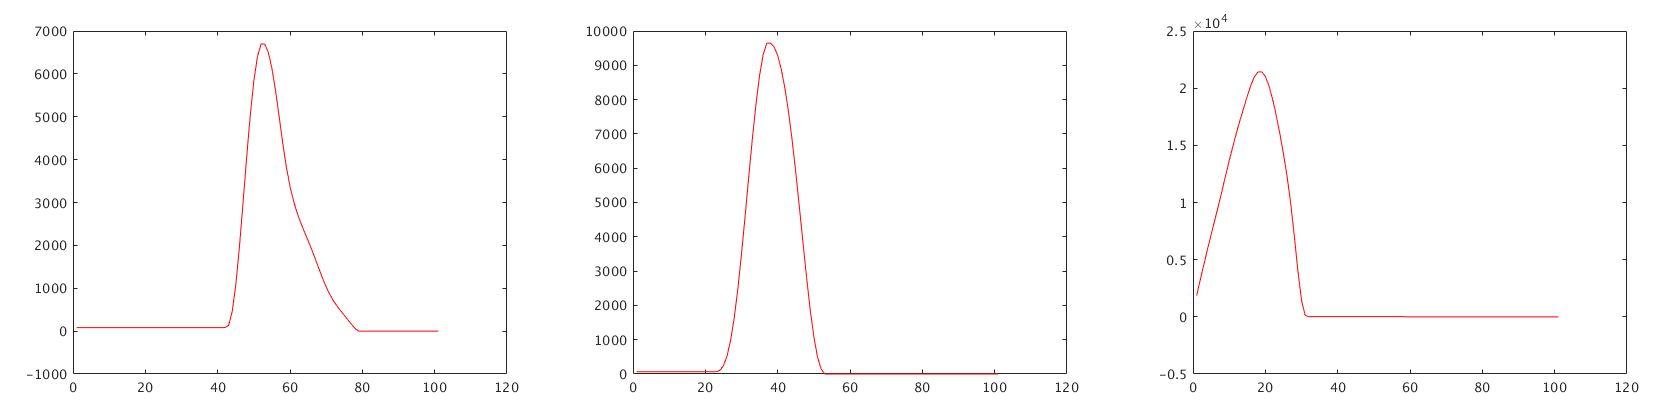
\includegraphics[width=160mm]{figs/sensors_perfect_chanall.png}
	\caption{Actual sensors (blue) and predicted sensors (red) for the three 
        channels: red (left), green (center), blue (right). Note that the match 
        is so good that the predicted sensors completely cover the actual sensors. 
        In an earlier version of the program, this was performed after rounding 
        to ints, which introduced some noise and allowed both actual and 
        predicted sensor curves to be visible.}
\end{figure}

\begin{figure}[!ht]
	\centering
	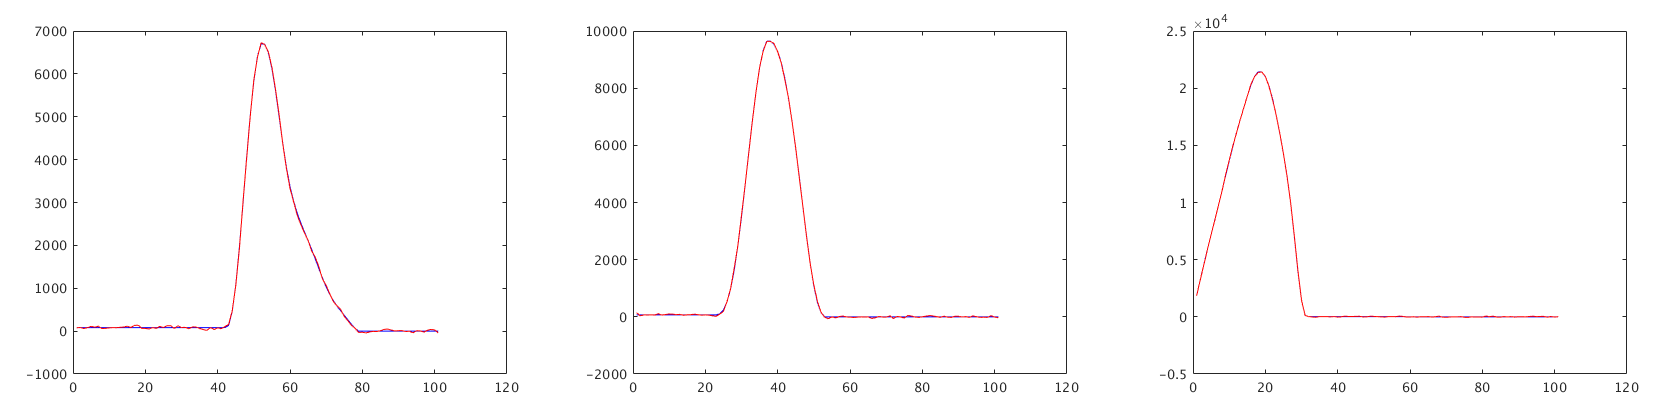
\includegraphics[width=160mm]{figs/sensors_introunded_chanall.png}
	\caption{The same curves by predicting after int rounding. Notice the 
        increased error due to the decreased precision.}
\end{figure}



The error values were as follows (for the non-int-rounded version):

\begin{tabular}{r | c c c}
                    & Red      & Green     & Blue      \\
    Sensor RMSE     & 7.51e-11 & 1.033e-10 & 2.906e-10 \\
    Output RGB RMSE & 3.78e-13 & 5.32e-13  & 1.442e-12 \\
\end{tabular}

\section{(\#3) Adding Gaussian Noise}

Perfect output like that of above is not very realistic, so we instead explore output with Gaussian 
noise. First, we randomly compute values from a normal distribution with mean 0 
and standard deviation 10, then, we add those values to the computed RGB values 
above. Like before, we pretend that we don't have the original sensor sensitivities, 
so we use the pseudoinverse method to find the least-squared-error solution The 
plots of the actual sensors and predicted sensors is below.

\begin{figure}[!ht]
	\centering
	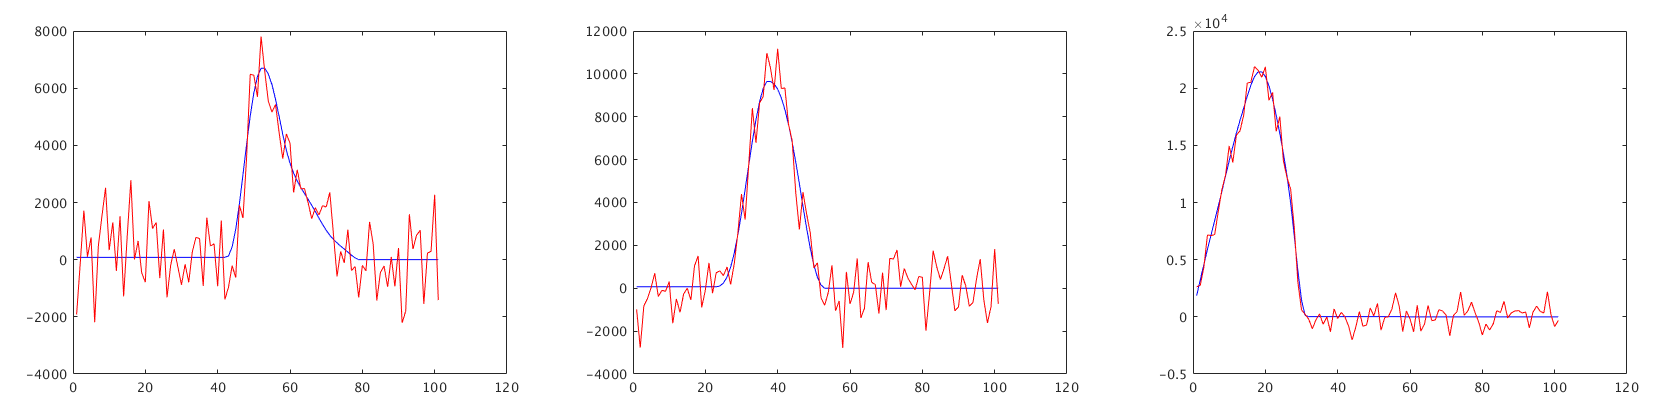
\includegraphics[width=160mm]{figs/sensors_noise_stddev10_unclipped_chanall.png}
	\caption{When we add Gaussian noise with standard deviation 10, the predicted 
        sensors are much noisier as well. However, they still roughly follow the 
        sensor curves.}
\end{figure}

And the accompanying errors:

\begin{tabular}{r | c c c}
                    & Red    & Green  & Blue   \\
    Sensor RMSE     & 1038.2 & 996.3  & 874.1  \\
    Output RGB RMSE & 2.7434 & 2.7259 & 2.3788 \\
\end{tabular}

However, we can also clip RGB to be within the range [0, 255], and this is much 
closer to reality, as images normally store RGB as 8-bit unsigned integers. Before 
looking at the plots, I would guess that the spectra most likely to be clipped 
will be spectra with a high value at either the peak or the tails of the sensor 
sensitivity curves. Thus, I would expect the predicted sensor curves to exhibit 
more noise at the tails and peak after clipping. Let's take a look:


\begin{figure}[!ht]
	\centering
	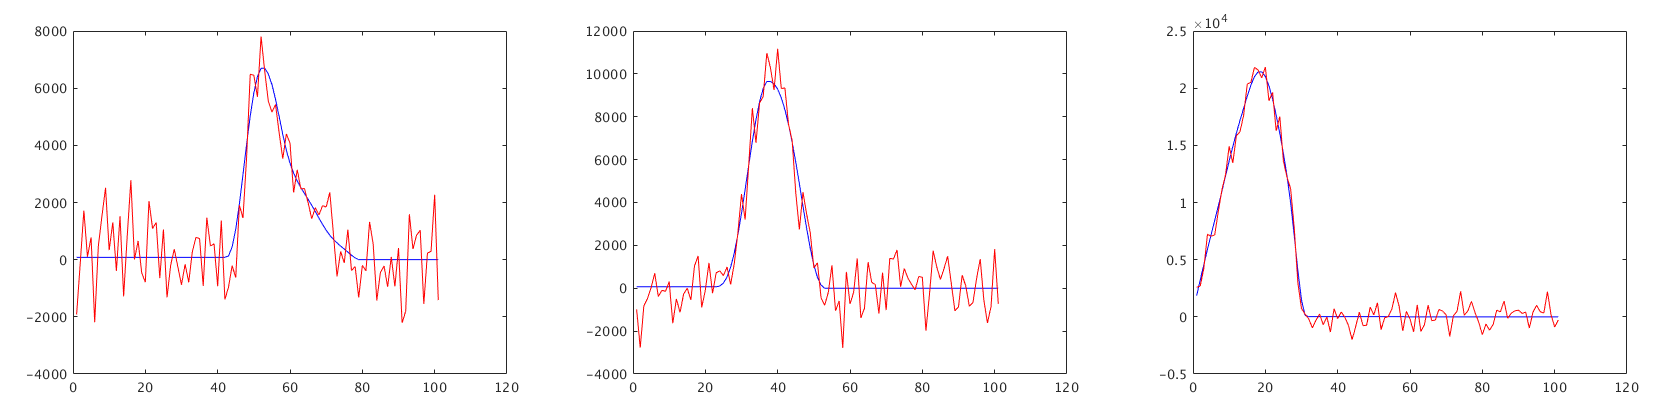
\includegraphics[width=160mm]{figs/sensors_noise_stddev10_clipped_chanall.png}
	\caption{Here, we clip the output RGBs to be in range [0, 255] to more 
        closely resemble reality and visualize the output sensors.}
\end{figure}

And the accompanyign errors:

\begin{tabular}{r | c c c}
                    & Red    & Green  & Blue   \\
    Sensor RMSE     & 1038.2 & 996.3  & 880.1  \\
    Output RGB RMSE & 2.7434 & 2.7259 & 2.3895 \\
\end{tabular}

It turns out the noise plots and the errors are very similar versus the 
unclipped data. In this case, this is probably indicative that there are very 
few color values close to the extremes. Remember that we need both an extreme 
value and Gaussian noise in the right direction to push it over the boundary.

\section{(\#4) Exploring Higher Noise Levels}

The noise does add a significant amount of jitter to the predicted sensor 
curves, but we should also explore what happens when we increase the noise 
level. In general, a higher noise level \textit{should} increase the difference 
between the unclipped error and clipped error, as more values are pushed out of 
bounds. In addition, it should make the resultant sensor curves even more jittery 
and obliterate more and more structure from those sensor curves until it is 
overcome completely by noise. Let's take a look at the graphs for noise with 
standard deviation 50 (both unclipped and clipped) and noise with standard 
deviation 100 (both unclipped and clipped), then at the chart 
of errors for all standard deviations in 10:10:100.

\begin{figure}[!ht]
	\centering
	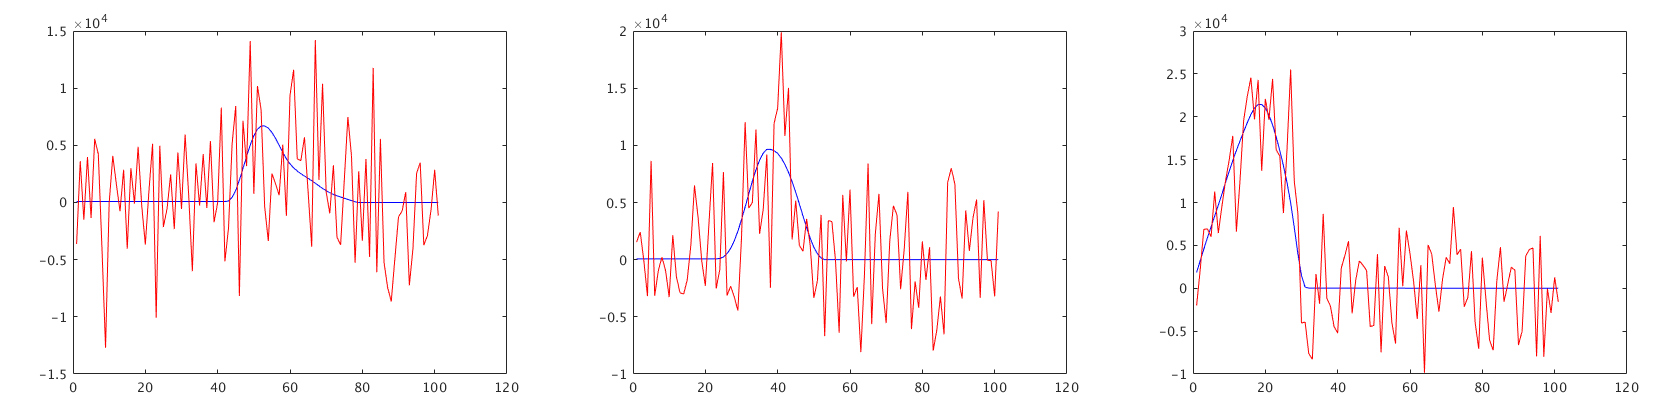
\includegraphics[width=160mm]{figs/sensors_noise_stddev50_unclipped_chanall.png}
	\caption{Actual and predicted sensors with noise of standard deviation 50, unclipped.}
\end{figure}

\begin{figure}[!ht]
	\centering
	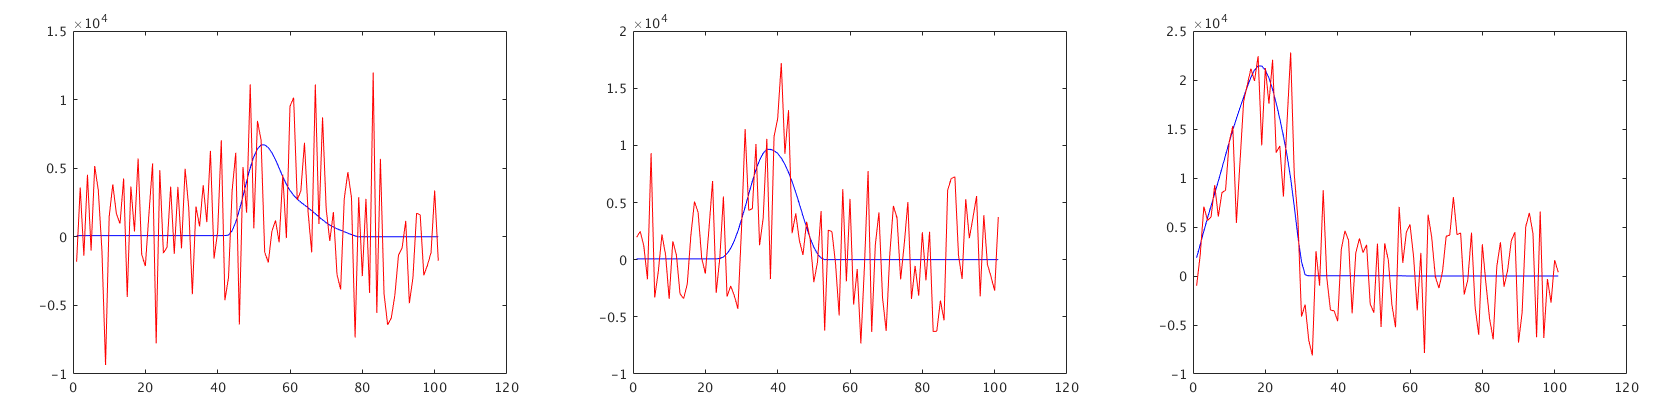
\includegraphics[width=160mm]{figs/sensors_noise_stddev50_clipped_chanall.png}
	\caption{Actual and predicted sensors with noise of standard deviation 50, clipped between [0, 255].}
\end{figure}

\begin{figure}[!ht]
	\centering
	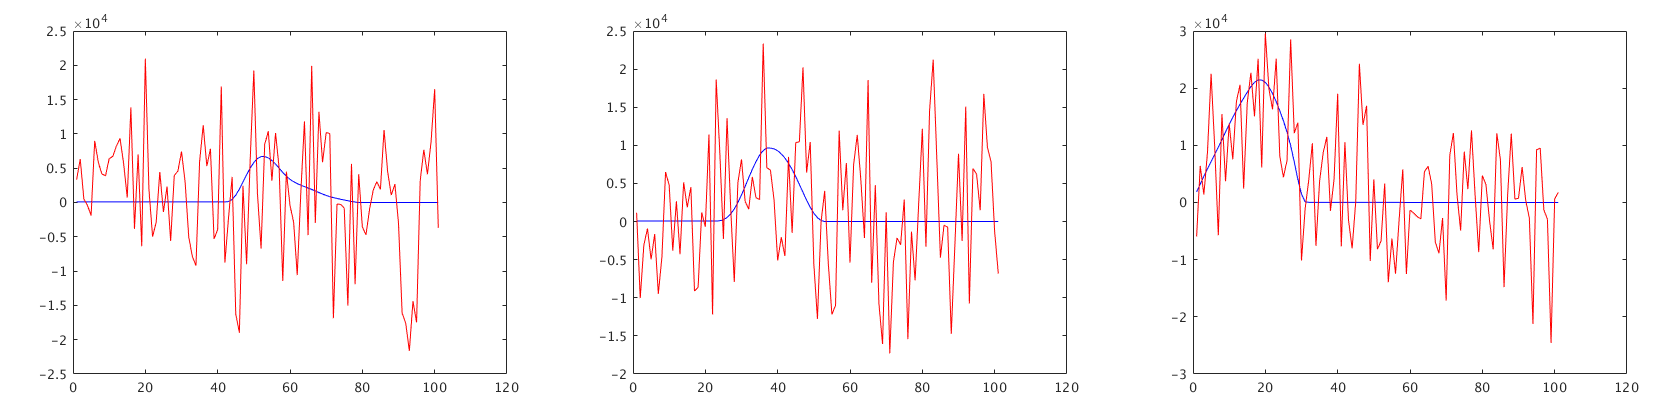
\includegraphics[width=160mm]{figs/sensors_noise_stddev100_unclipped_chanall.png}
	\caption{Actual and predicted sensors with noise of standard deviation 100, unclipped.}
\end{figure}

\begin{figure}[!ht]
	\centering
	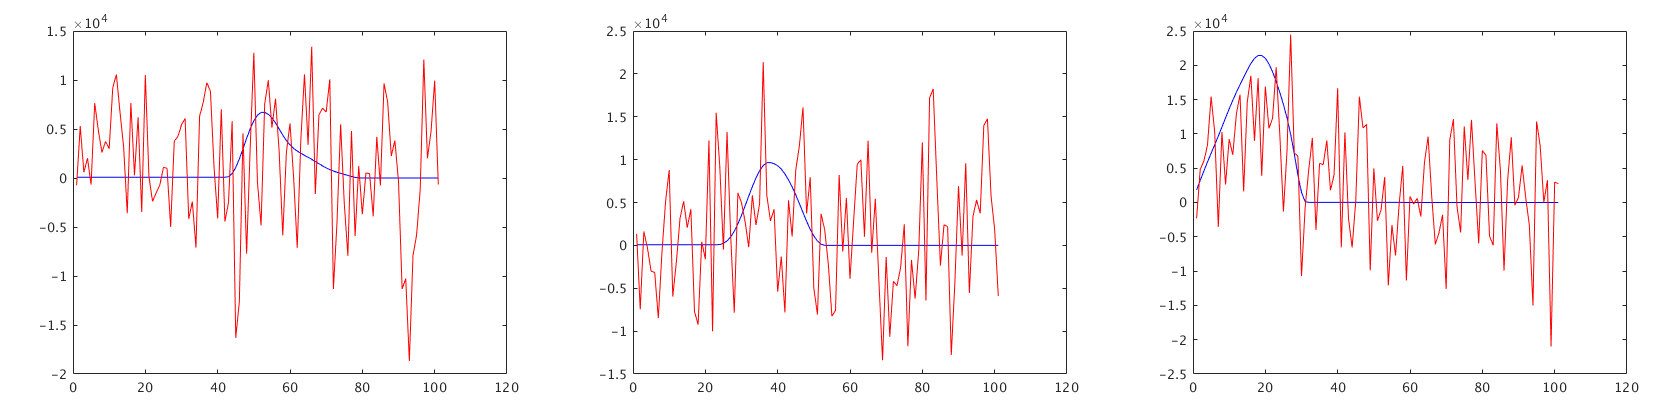
\includegraphics[width=160mm]{figs/sensors_noise_stddev100_clipped_chanall.png}
	\caption{Actual and predicted sensors with noise of standard deviation 100, clipped between [0, 255].}
\end{figure}

Selected errors.:

\begin{tabular}{r | r r r r}
                  & unclipped sensor RMSE & unclipped data RMSE & clipped sensor RMSE & clipped data RMSE   \\
    $\sigma = 0$  &    0.0 &  0.0000 &    0.0 &  0.0000 \\
    $\sigma = 1$  &  948.4 &  2.5089 &  949.1 &  2.5108 \\
    $\sigma = 2$  & 1887.3 &  4.9134 & 1877.8 &  4.8880 \\
    $\sigma = 3$  & 2930.7 &  7.7992 & 2873.6 &  7.6749 \\
    $\sigma = 4$  & 3596.6 &  9.5844 & 3425.1 &  9.3724 \\
    $\sigma = 5$  & 4685.1 & 12.4859 & 4227.3 & 11.6164 \\
    $\sigma = 6$  & 5473.3 & 14.5444 & 4810.9 & 13.6015 \\
    $\sigma = 7$  & 6728.6 & 18.0828 & 5574.2 & 17.6235 \\
    $\sigma = 8$  & 7566.5 & 19.7145 & 6126.3 & 18.8280 \\
    $\sigma = 9$  & 7925.0 & 21.6100 & 6177.6 & 21.9431 \\
    $\sigma = 10$ & 8797.3 & 23.4598 & 7276.3 & 25.0892 \\
\end{tabular}

\subsection{Discussion}

The error appears to increase linearly with sigma. The plots also show that 
sigma causes the predicted sensors to be much more jittery. The curves even start 
to be harder to pick out among the jitter. As expected, more noise does increase 
the chance of clipping. However, clipping has a strange effect on the respective 
errors. While clipping increases the data errror, it decreases the sensor error. I 
am a little stumped at this result, and I have double-checked my code to verify 
that it's doing what I think it's doing. If the results are correct, we could 
hypothesize as to why clipping would reduce the sensor error. One way to think 
of it might be to think in terms of our original data range and how we scaled it. 
At the beginning of the program, we scaled our random spectra values by a constant $ k $ at 
the beginning of the program to ensure that the RGB outputs would always be in 
range [0, 255]. Returning to our noisy samples, if we clip a negative number to 
0, it \textit{must} be closer to its original value because of that scaling 
constant $ k $. I'm still stumped as to why the data error is larger, though.

\section{(\#5) Gamma Correction}

Here, we simply solve the gamma correction equation for $\gamma$:

$$
f(x) = 255 (\frac{x}{255})^{\frac{1}{\gamma}}
$$

Substituting for x, and f(x):

$$
127 = 255 (\frac{80}{255})^{\frac{1}{\gamma}}
$$
$$
\frac{127}{255} = \frac{80}{255}^{\frac{1}{\gamma}}
$$
$$
log(\frac{127}{255}) = \frac{1}{\gamma} log(\frac{80}{255})
$$
$$
\gamma = \frac{log(\frac{80}{255})}{log(\frac{127}{255})} = 1.6630
$$

\section{(\#6) Problems Using the Pseudoinverse on Real Data}

\begin{figure}[!ht]
	\centering
	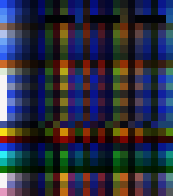
\includegraphics[width=80mm]{figs/real_data.png}
	\caption{This is my best guess of an image of the given real-world RGB 
        values. I wanted to visualize it a little better, so I guessed at the 
        height and width.}
\end{figure}

When using this technique on real world data, we find that it performs very poorly.

\begin{figure}[!ht]
	\centering
	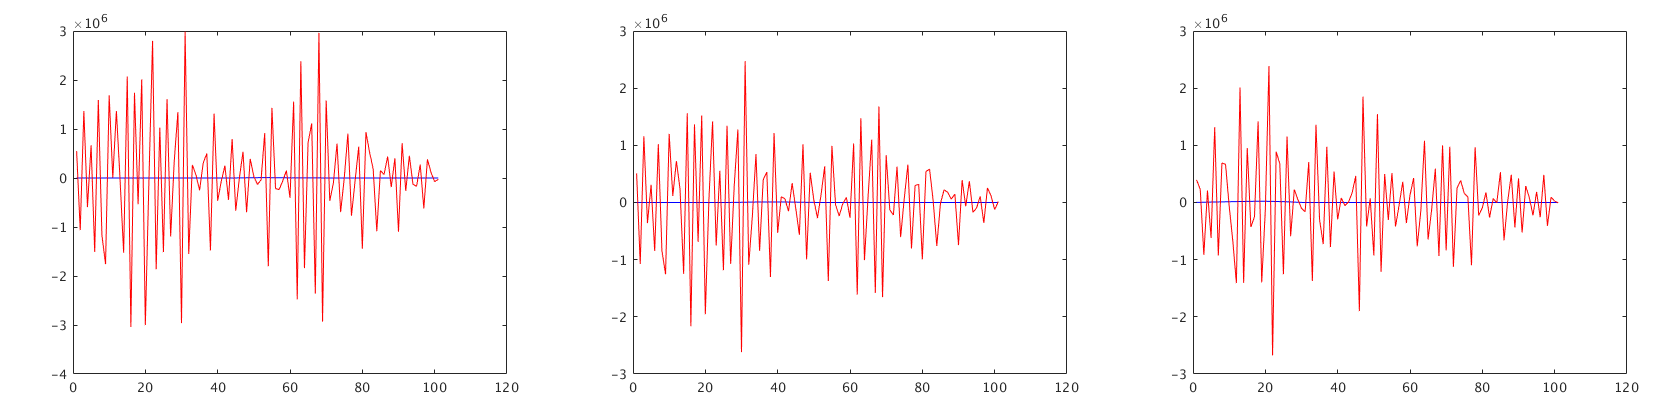
\includegraphics[width=160mm]{figs/sensors_unconstrained_chanall.png}
	\caption{Extremely poor performance of predicted sensor curves. The noise is 
        so bad that the actual sensor curves are dwarfed and appear close to 0.}
\end{figure}

The errors are extremely high as well:

\begin{tabular}{r r}
    Sensor RMSE & Data RMSE \\
    1.0138e6    & 5.7426    \\
\end{tabular}

\subsection{Discussion}

Consider the case where none of the spectra samples have a non-zero value in a 
particular spectral bin. In this case, the matrix might as well be 100 columns 
instead of 101! Thinking in terms of linear algebra, if we find that our 
spectral samples lie on some subspace of the actual space of possible spectral 
samples, we have a degenerative matrix. The basis of such a matrix is less 
than the dimensionality. For a normal n-by-n matrix, this would mean that the 
matrix can't be inverted. In the case of our pseudo-inverse, maybe something 
similar happens. While we can still take the pseudo-inverse, perhaps it's no 
longer useful.

\section{(\#7) Constrained Least Squared Error}

If we constrain sensors to only have positive responses, the prospect is much 
less bleak. Here, we must use a different technique, adding a constraint 
expression (using quadprog in MATLAB). The resultant sensors are still very spikey, but the spikes tend to 
be near the actual sensor peaks.

\begin{figure}[!ht]
	\centering
	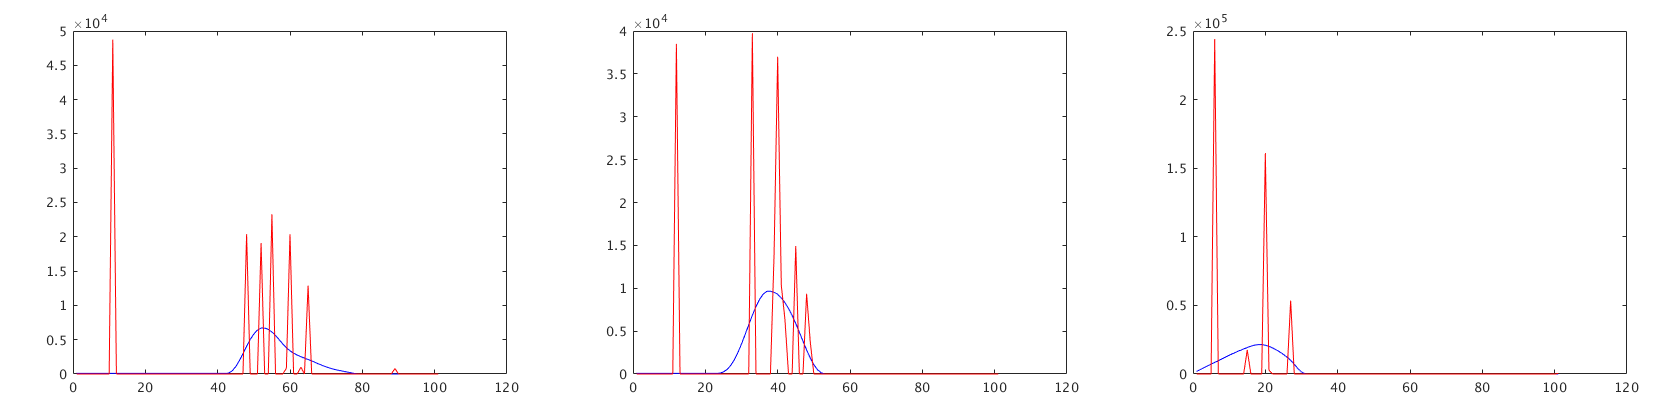
\includegraphics[width=160mm]{figs/sensors_nonzero_chanall.png}
	\caption{Predicted sensor curves when we constrain them to be 0 or positive. 
        The results are much better, and the spikes tend to be near the actual 
        sensor peaks. However, there are still several outlier spikes that are 
        nowhere near the peaks.}
\end{figure}

\section{(\#8) Smooth, Non-negative Predictions}

We can also attempt to make the curves smoother to get rid of the spikes above. 
We can do so rather cleverly by concatenating the following matrix at the bottom 
of our spectra matrix:

$$
M = \begin{bmatrix}
1      & -1     &      0 &        & \cdots & 0 & 0 \\
0      &  1     &     -1 &      0 & \cdots & 0 & 0 \\
\vdots & \vdots & \vdots & \vdots & \ddots & 0 & 0 \\
0      & \cdots &        &        & \cdots & 1 & -1
\end{bmatrix}
$$

Now, this essentially represents the difference between adjacent spectral 
response buckets for our sensors. We want each of these differences to be small, 
so we append 0's at the bottom of the RGB output matrix. Finally, we multiply M 
by a constant $\lambda$ to allow us to control the smoothness. Several different 
plots are presented for different lambda values. I think a value of $\lambda = 0.01$ 
matches the original sensors pretty well.

\begin{figure}[!ht]
	\centering
	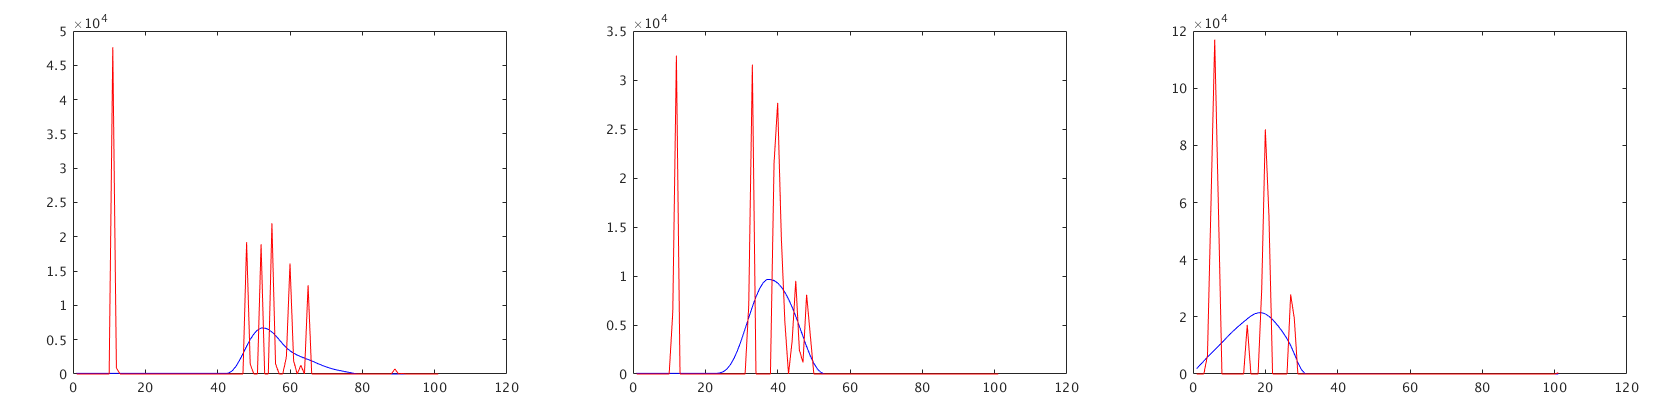
\includegraphics[width=160mm]{figs/sensors_smooth_lam0_0001_chanall.png}
	\caption{lambda (smoothing constant) = 0.0001 (very low)}
\end{figure}

\begin{figure}[!ht]
	\centering
	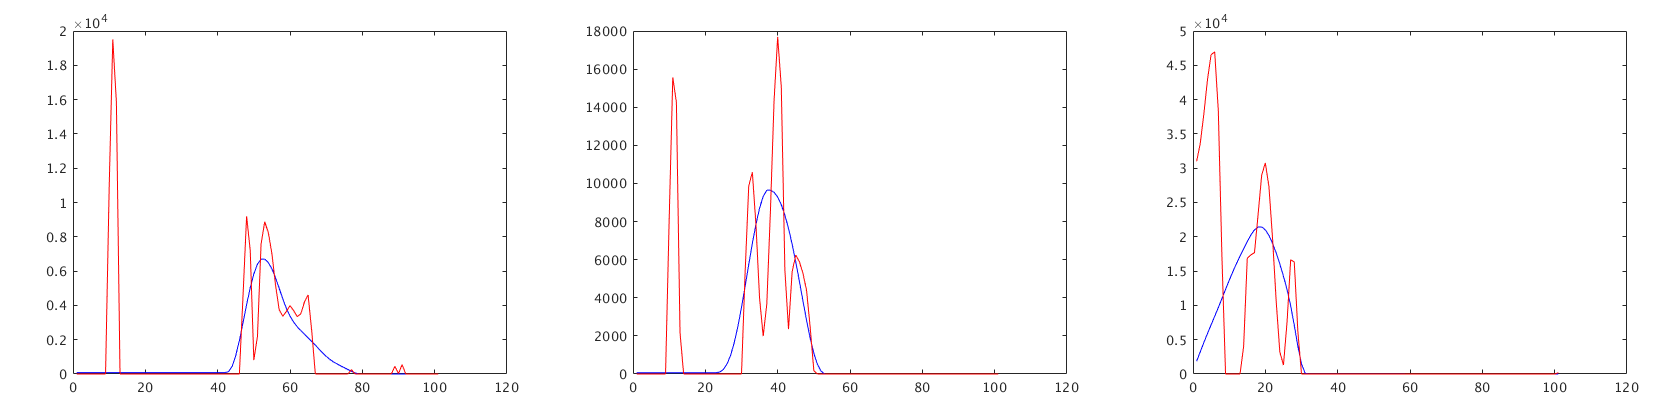
\includegraphics[width=160mm]{figs/sensors_smooth_lam0_0010_chanall.png}
	\caption{lambda (smoothing constant) = 0.001 (low)}
\end{figure}

\begin{figure}[!ht]
	\centering
	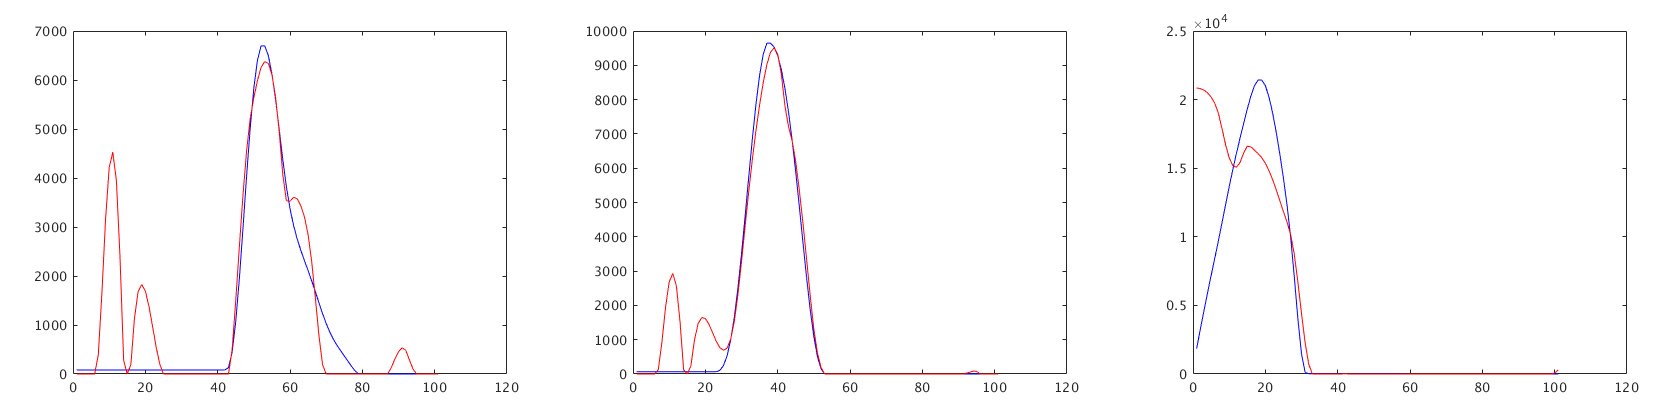
\includegraphics[width=160mm]{figs/sensors_smooth_lam0_0100_chanall.png}
	\caption{lambda (smoothing constant) = 0.01 (about right)}
\end{figure}

\begin{figure}[!ht]
	\centering
	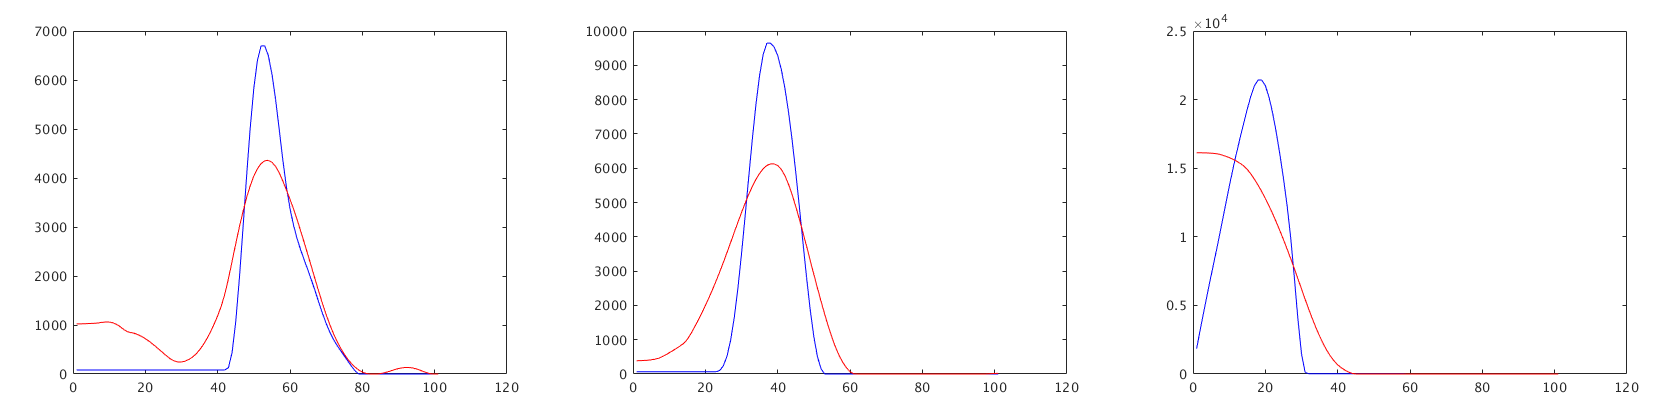
\includegraphics[width=160mm]{figs/sensors_smooth_lam0_1000_chanall.png}
	\caption{lambda (smoothing constant) = 0.1 (high)}
\end{figure}

\begin{figure}[!ht]
	\centering
	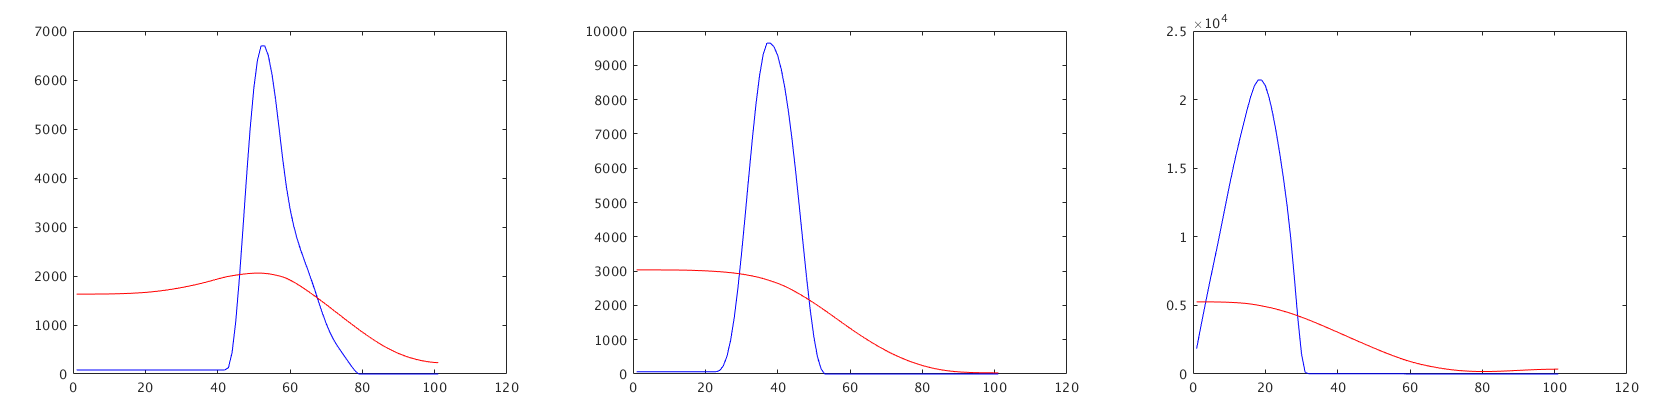
\includegraphics[width=160mm]{figs/sensors_smooth_lam1_0000_chanall.png}
	\caption{lambda (smoothing constant) = 1 (very high)}
\end{figure}

\subsection{Discussion}

We can turn the $\lambda$ knob so that the curves are as smooth or jagged as we want, but, 
in a real world case, we might not have the training data (actual sensor curves) 
to compare against. In that case, how would we know a good value for $\lambda$?

\end{document}